% MDPI Cryptography revised submission package, verified 18 September 2026.
% Pin the template's visible submission-version date to the date of the
% authoritative PDF submitted to the journal.
\year=2026 \month=9 \day=17
\documentclass[cryptography,article,submit,oneauthor]{Definitions/mdpi}

\firstpage{1}
\makeatletter
\setcounter{page}{\@firstpage}
\makeatother
\pubvolume{1}
\issuenum{1}
\articlenumber{0}
\pubyear{2026}
\copyrightyear{2026}
\datereceived{}
\daterevised{}
\dateaccepted{}
\datepublished{}

\newcommand{\T}{\mathsf{T}}
\rightlinenumbers
\Title{Structural Limits of Orientation Scheduling in Byte-Local GF(2) Diffusion Layers}
\newcommand{\orcidauthorA}{0000-0003-3734-5478}
\Author{Porter E. Coggins, III $^{1,*}$\orcidA{}}
\AuthorNames{Porter E. Coggins, III}
\address{$^{1}$ \quad Department of Professional Education, Bemidji State University, Bemidji, MN 56601, USA; porter.coggins@bemidjistate.edu}
\corres{Correspondence: porter.coggins@bemidjistate.edu}

\abstract{Orientation scheduling varies linear coefficients across rounds while preserving byte locality, invertibility, the branch-number floor, and the surrounding substitution-permutation network. For independently applied $8\times8$ invertible maps over $\mathrm{GF}(2)$, active-byte support is invariant at the matrix step; this elementary block-diagonal fact is used here as a screening invariant rather than as a new algebraic theorem. The restriction does not extend to linear layers whose coefficients couple byte positions. Under the standard Markov-cipher model, a 128-state transfer computation over a deterministic panel of 256 matrix contexts finds a small separation between temporally constant and round-dependent schedules. At 16 rounds the oracle-maximized geometric-mean class probabilities are about $2^{-78.2}$ to $2^{-78.5}$, and the rotor-minus-static periodic-rate contrast is $0.00881$ bits/round on the primary panel. Prefix and independently labelled panel checks give contrasts of the same order. The one-step ordering reverses under the periodic operator, an observation consistent with temporal-alignment effects but not sufficient to identify a unique mechanism. Reduced-round fixed-key calibration also shows that deviations from the Markov surrogate can be much larger than the schedule separation. The numerical difference is therefore resolvable but numerically small within the transfer model and is not presented as a fixed-key security advantage. The aggregate weight-one class exceeds the best individual trail by about $2^{28}$ in mean log-domain gap. The resulting design lesson is structural: coefficient diversity can change local transition quality and ordering, but within a byte-local layer it cannot substitute for diffusion width.}
\keyword{orientation scheduling; diffusion layers; differential cryptanalysis; linear cryptanalysis; Markov-cipher model; matched controls}
\MSC{94A60; 94B05; 15B33; 11T71}

\begin{document}
\section{Introduction}\label{sec:1}
Substitution-permutation networks (SPNs) obtain security from repeated interaction between nonlinear substitution and linear or permutation-based diffusion \cite{ref1}, \cite{ref2}, \cite{ref4}, and \cite{ref21}. The present study examines one narrowly defined diffusion-layer question arising from earlier Hill-matrix work: whether publicly changing the orientation of a binary matrix across rounds and byte positions contributes meaningful diffusion when that matrix is applied independently to each byte \cite{ref10} and \cite{ref11}.

\subsection{Research Question and Structural Hypothesis}\label{sec:1-1}
\noindent\textbf{Research question.} Holding the seed matrices, round keys, nonlinear layer, whole-state rotation, and routing permutation fixed, does changing only the public orientation schedule of byte-local invertible $8\times8$ matrices over $\mathrm{GF}(2)$ improve differential diffusion relative to a static orientation?

Orientation scheduling is a plausible intervention because it preserves invertibility and the imposed branch-number floor while changing coefficient placement inside a byte. Across rounds, those changes can alter the difference patterns presented to subsequent S-boxes. The structural screening question is whether that variation also changes the number of active byte positions. For independently applied byte-local maps it cannot: there is no coefficient path from one byte to another at the matrix step. The contribution is therefore not the algebraic difficulty of that observation, but its use to separate coefficient diversity from diffusion width and to define the minimum-support class in which any residual scheduling effect must be transition-level rather than support-growth-level.

The restriction is essential. Nothing in the support-invariance statement applies to a linear layer whose coefficients couple distinct byte positions. Such cross-byte layers are discussed only as a boundary to the present result.

\subsection{Why the Structural Limitation Matters}\label{sec:1-significance}
Wide-trail reasoning links resistance to differential and linear propagation to the number of nonlinear components forced active by the linear layer \cite{ref21,ref5}. A design may vary matrices, coefficients, or orientations from round to round without increasing that active-component count. For a byte-local layer, coefficient changes can affect local differential probabilities and correlations, but they do not themselves enlarge byte support. The engineering screen suggested by this paper is therefore simple: before paying implementation or analysis cost for a varying linear rule, determine whether the variation changes support geometry at the symbol width feeding the nonlinear layer. If it does not, any benefit must come from coefficient-sensitive transition ordering rather than from a stronger active-S-box bound.

\subsection{Main Findings}\label{sec:1-2}
The byte-local support statement is an elementary consequence of block-diagonal structure and is used as a causal screening invariant. The new analysis is the finite-state weight-one transfer model built around that invariant, its schedule comparison over deterministic matrix contexts, and the separation of aggregate class probability from best-trail probability.

Within the Markov-cipher transfer model, the periodic rotor-minus-static decay-rate contrast is $0.00881$ bits/round on the 256-context primary panel. Prefix checks give $0.01731$, $0.01231$, $0.00881$, and $0.01037$ bits/round for the first $64$, $128$, $256$, and $512$ contexts, while an independently domain-separated 256-context panel gives $0.00939$ bits/round. The paired context-level distributions are broad, so these values are presented as model-internal panel summaries rather than universal parameters.

At 16 rounds, the per-context oracle maximum over the 128 starting weight-one differences has mean log$_2$ probability $-78.211$ for static and $-78.515$ for rotor. These are log-domain summaries, equivalently geometric-mean probabilities, not arithmetic probability means. The corresponding arithmetic-mean probability exponents are $-78.047$ and $-78.455$. The oracle maximum is a conservative structural diagnostic because the matrices are secret functions of the master key; it is not an operational attacker-selected differential. A fixed preselected start (bit 0) gives arithmetic-mean exponents $-79.365$ and $-79.638$ for static and rotor, respectively.

The one-step ordering reverses under the periodic operator: static has a slightly larger phase-averaged one-step decay than rotor but a smaller periodic decay. This rules out a simple explanation based on uniformly better one-step transitions. Temporal alignment is a natural interpretation, especially because static and position-only schedules are temporally constant at a fixed byte position, but the four-schedule comparison does not identify a unique noncommutative mechanism.

The model result is numerically stable but model-dependent. An independent direct-eigenvalue and long-horizon dynamic check agrees with the implemented power iteration to below $9\times10^{-16}$ bits/round on a validation subset, including reducible period products. By contrast, a reduced-round fixed-key calibration shows context/start deviations from the Markov predictions that are much larger than the $0.009$-bit/round schedule separation. The schedule separation is therefore resolvable but numerically small within the surrogate model and is not interpreted as a fixed-key security gain.

\subsection{Scope, Claim Status, and Adversary Model}\label{sec:1-3}
The historical Hill-Enigma-SPN construction is retained only as a fully specified 128-bit experimental harness. It is not proposed as a deployment-ready cipher or as a replacement for AES. The orientation rule is public and contains no entropy. The sixteen accepted seed matrices are deterministic functions of the master key and are treated as secret internal components of the harness. Consequently, a per-context maximum over starting differences assumes knowledge not available to an attacker who does not know the key; throughout this paper it is labelled an \emph{oracle-maximized structural diagnostic}, not an attack probability.

The status of the principal claims is deliberately separated. Byte-local support invariance, invertibility preservation under orientation, the DDT column-sum identity, and the Parseval identity are elementary or standard facts specialized to this setting. The 128-state scheduled transfer system, its 256-context numerical evaluation, the one-step/periodic ordering reversal, the panel sensitivity checks, and the class-versus-single-trail gap are analyses or numerical findings reported here. All reported rate magnitudes are harness-specific and must be recomputed for another S-box, matrix family, routing rule, or state-motion schedule.

Relative to earlier Hill-derived work \cite{ref10,ref11,ref22}, the present paper uses the orientation operation as a public ablation variable rather than as secret transformation material, introduces the weight-one finite-state transfer analysis, and studies aggregate low-support differential recurrence. The earlier multidimensional Hill SPN \cite{ref22} uses fixed cross-byte MDS mixing and contains no orientation-schedule comparison.

The contributions are therefore: (i) formalizing the byte-local support screen in the specific context of orientation scheduling; (ii) connecting that screen to the weight-one recurrence class; (iii) specifying and evaluating the resulting Markov transfer system, including selection and averaging conventions; (iv) separating aggregate class mass from best individual trails; and (v) delimiting what the model result does and does not imply for a fixed keyed permutation.

\begin{figure}[t]
\centering
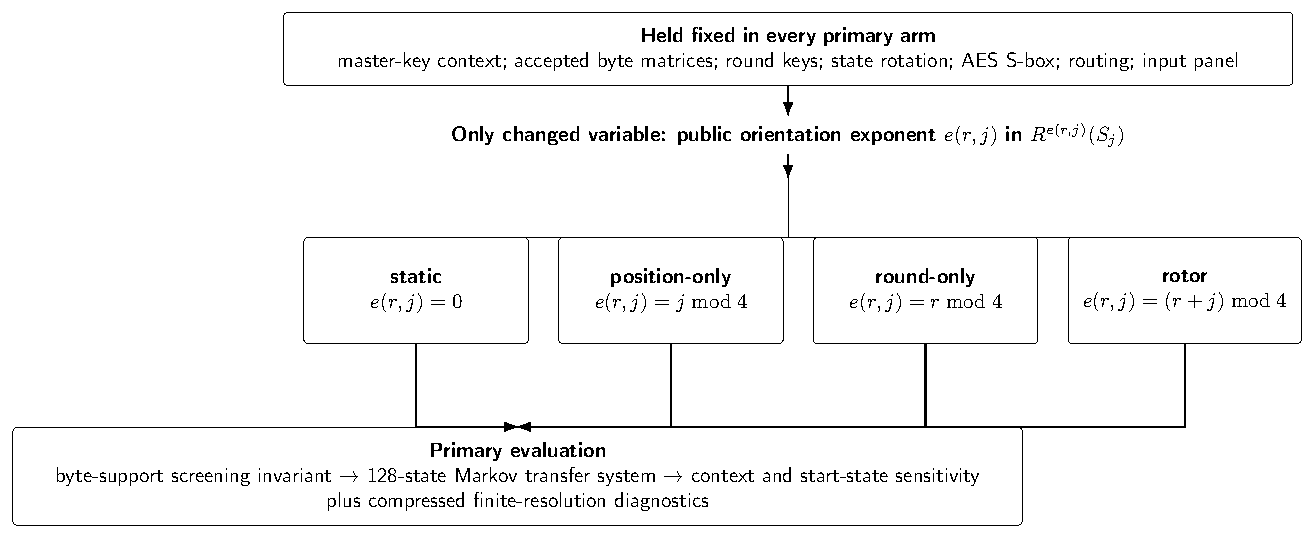
\includegraphics[width=0.97\textwidth]{Fig1}
\caption{Matched primary design. All components are held fixed except the public orientation exponent. The separate cross-byte MDS example is exploratory, changes several variables simultaneously, and is documented in the Supplementary Material.}\label{fig:design}
\end{figure}

\subsection{Organization}\label{sec:1-5}
Section~\ref{sec:2} places the question in the Hill-matrix and SPN diffusion literature. Section~\ref{sec:3} develops the byte-local support result, motivates the weight-one minimum-support class, and gives the differential and linear transfer analysis. Section~\ref{sec:4} specifies the experimental harness. Section~\ref{sec:primary} gives the compressed matched corroboration and exploratory cross-byte boundary conclusion, with detailed diagnostics moved to the supplement. Section~\ref{sec:6} discusses the design implications, limitations, and open questions.
\section{Related Work and Structural Context}\label{sec:2}
\subsection{Hill-Matrix Variation and Orientation}\label{sec:2-1}
The classical Hill cipher uses invertible matrix multiplication as a linear transformation \cite{ref8} and \cite{ref9}. Its linearity motivated variants that change the key matrix between messages, combine Hill multiplication with additional transformations, or alter matrix structure; representative examples include Saeednia \cite{ref26}, Ismail et al. \cite{ref28}, and Toorani and Falahati \cite{ref20}. Coggins and Glatzer \cite{ref10} and Coggins \cite{ref11} used matrix-element rotations explicitly to vary Hill-derived transformations. Those two citations are the direct source of the orientation operation studied here. The present paper does not treat orientation as secret key material; it asks whether using the orientations as a public schedule changes diffusion when embedded in an otherwise fixed SPN.

A closer architectural predecessor is the multidimensional Hill SPN of Coggins \cite{ref22}, which uses global MDS matrices over $\mathrm{GF}(2^8)$. That construction and the present harness differ in the property under investigation: the former uses fixed cross-byte mixing, whereas the present experiment deliberately uses byte-local $8\times8$ binary maps so that orientation scheduling can be isolated as an experimental variable.

\subsection{SPN Diffusion and Branch Number}\label{sec:2-2}
The wide-trail strategy relates linear-layer diffusion to lower bounds on active nonlinear components across rounds \cite{ref21}. Branch number is therefore useful only at the algebraic granularity at which the linear map operates. AES MixColumns, for example, is an MDS map across four bytes over $\mathrm{GF}(2^8)$ with branch number five \cite{ref5} and \cite{ref6}; SHARK similarly uses an MDS layer over byte symbols \cite{ref24}. By contrast, the byte-local test layer applies independent maps to individual bytes over $\mathrm{GF}(2)$. Its branch-number floor constrains bit spreading \emph{inside} a byte and is not a cross-byte wide-trail guarantee. Differential and linear branch numbers of binary matrices are treated in the terminology of Sarkar and Syed \cite{ref18}.

The distinction is summarized in Table~\ref{tab:context}. It is central to the research question: if an orientation schedule is to affect spatial diffusion, the linear layer must expose positional structure that can actually be changed by orientation.

\begin{table}[t]
\caption{Structural context for the diffusion layers discussed in this study. The comparison is algebraic, not a security or performance ranking.}\label{tab:context}
\centering\small
\begin{tabular}{@{}llll@{}}
\toprule
Layer & Domain & Mixing width & Role here \\
\midrule
Byte-local scheduled layer & $\mathrm{GF}(2)$ & 1 byte & mechanism under test \\
AES MixColumns \cite{ref5} and \cite{ref6} & $\mathrm{GF}(2^8)$ & 4 bytes & cross-byte reference \\
Cross-byte boundary setting & $\mathrm{GF}(2^8)$ & 4 bytes & boundary experiment \\
\bottomrule
\end{tabular}
\end{table}

\subsection{Round-Varying and Structurally Diverse Layers}\label{sec:2-4}
Round-varying public linear layers are an established design choice, but variation itself is not a security argument. LowMC uses independently generated dense binary matrices across rounds \cite{ref52}, and its cryptanalysis treats those matrices as fixed public instance data whose interaction with the nonlinear layer must be analyzed \cite{ref53}. Rasta instead uses pseudorandomly generated affine layers, while Dasta studies a fixed-linear-layer alternative and thereby isolates the cost and role of that variation \cite{ref58,ref59}. These constructions are not matched controls for the present harness because their linear layers span the full state, but they illustrate the relevant design distinction: changing a linear rule over time and increasing the support width of that rule are separate choices.

Structural diversity also arises outside matrix scheduling. Cellular-automata-based S-box constructions, for example, vary local update structure rather than merely permuting coefficients inside a fixed byte-local support \cite{ref60}. Such work is relevant here because it changes the locality mechanism itself, which is precisely the variable held fixed in the present orientation experiment.

\subsection{Differential Aggregation and Persistent Low-Support Structure}\label{sec:2-5}
Differential cryptanalysis distinguishes individual characteristics from aggregate differentials, and the probability mass of many trails can differ substantially from that of the best single trail \cite{ref54,ref62}. Ankele and K\"olbl emphasize the gap between active-S-box bounds and achievable differential behavior in concrete block ciphers \cite{ref61}. Persistent structural subsets are also central to invariant-subspace attacks, although the mechanisms differ from the substochastic recurrence class considered here \cite{ref63}. These lines of work motivate reporting both the best single trail and the aggregate weight-one class rather than treating one characteristic as a complete description of low-support behavior.

\subsection{Gap Addressed}\label{sec:2-6}
Existing work shows that round-varying linear maps, global diffusion, and structural diversity can be useful ingredients, but it does not answer the narrower causal question posed here: what remains when only the orientation of a byte-local binary map is varied while support width is held fixed? The present experiment therefore compares schedule variants over identical components and explicitly separates an elementary support invariant from the coefficient-sensitive transfer quantities that remain. A separate cross-byte MDS experiment is retained only as an exploratory boundary example because it changes width, field, and matrix family simultaneously.
\section{Byte-Local Orientation Scheduling: Structural Analysis and Transfer Model}\label{sec:3}
This section defines the scheduled binary layer and isolates the structural property relevant to the research question. The central distinction is between \emph{intra-byte} bit spreading, which the $8\times8$ matrices can provide, and \emph{cross-byte} support growth, which they cannot provide on their own. A finite-state transition computation then quantifies the resulting weight-one differential class under an explicitly stated Markov-cipher model.\par
\subsection{Bit-Ordering Conventions (MSB-First)}\label{sec:3-1}
The reference implementation uses one MSB-first convention throughout. A byte $x$ is represented by $v(x)[i]=(x\gg(7-i))\mathbin{\&}1$; each matrix row is stored as a byte with the same bit order, and matrix-vector multiplication computes the parity of the row/input bitwise intersection. A 128-bit state is the big-endian sequence of 16 bytes, so \texttt{rotl128} rotates the corresponding big-endian integer and then repacks it as 16 bytes. Round indices in the key schedule are encoded as two-byte big-endian integers. These conventions are normative for reproducing the test vector; the supplementary implementation provides worked byte-level checks.\par
\subsection[Linear Maps and 8 x 8 Binary Matrices]{Linear Maps and 8\ensuremath{\times}8 Binary Matrices}\label{sec:3-2}
An 8\ensuremath{\times}8 matrix M \ensuremath{\in} GF(2)\textsuperscript{8}\textsuperscript{x}\textsuperscript{8} defines a linear map M: GF(2)\textsuperscript{8} \ensuremath{\rightarrow} GF(2)\textsuperscript{8}. Invertibility is equivalent to full rank over GF(2) and is verified by Gaussian elimination with MSB-first pivot selection.\par
The admissible seeds form a branch-number-filtered subset of $\mathrm{GL}(8,2)$; approximately 29\% of all $8\times8$ binary matrices are invertible \cite{ref12}. The 16 seeds are deterministic functions of the master key and add no independent entropy. Their role in this study is to provide matched local linear maps whose orientations can be scheduled without changing the underlying seed family.\par
\textbf{Granularity of the guarantee. }The branch-number condition used below is defined over eight bits within one byte. It must not be interpreted as the four-byte MDS branch-number guarantee of AES MixColumns.\par
\subsection{Branch Number as a Diffusion Metric}\label{sec:3-3}
\begin{Definition}[branch number]
For a linear map M: GF(2)\textsuperscript{n} \ensuremath{\rightarrow} GF(2)\textsuperscript{n}, B(M) = min\_\{x\ensuremath{\neq}0\} ( wt(x) + wt(Mx) ) \cite{ref5}. Since this depends only on Hamming weights it is independent of MSB/LSB convention. A lower bound on B(M) forces nontrivial spreading of any input difference. In the terminology of Sarkar \& Syed \cite{ref18}, B(M) is the differential branch number; the linear branch number is B(M\textsuperscript{T}), and the two need not coincide.
\end{Definition}

\subsection[Clockwise 90-degree Rotation: Algebra and Consequences]{Clockwise 90\ensuremath{^\circ} Rotation: Algebra and Consequences}\label{sec:3-4}
For M \ensuremath{\in} GF(2)\textasciicircum{}\{8\ensuremath{\times}8\}, define R(M) by R(M)\textsubscript{i}\textsubscript{j} = M\_\{(7-j), i\}. This permutes the 64 entries via the index map \ensuremath{\pi}: (i,j) \ensuremath{\mapsto} (j, 7-i) and satisfies R\textsuperscript{4}(M) = M.\par
\begin{Proposition}[Invertibility preservation]
With J the reversal (antidiagonal identity) permutation matrix, R(M) = M\textsuperscript{T}J. Hence R preserves invertibility over GL(8, 2): transpose preserves invertibility and right-multiplication by a permutation matrix preserves invertibility. Therefore M \ensuremath{\in} GL(8, 2) implies R(M) \ensuremath{\in} GL(8, 2) automatically. 
\end{Proposition}

\begin{Proposition}[Branch numbers of the four orientations]\label{prop:orientation-branch}
Because $R(M)=M^{\T}J$ with $J$ weight-preserving, the four orientations realize only the two branch numbers $B(M)$ and $B(M^{\T})$. Thus $B(M)\geq4$ and $B(M^{\T})\geq4$ are sufficient to guarantee the same floor for all four orientations.
\end{Proposition}
\begin{Definition}[admissible seed]
A seed $S$ is admissible when it is invertible and satisfies $B(S)\geq4$ and $B(S^{\T})\geq4$. By Proposition~\ref{prop:orientation-branch}, every orientation $R^k(S)$ is then invertible and has branch number at least four. The implementation checks all four orientations defensively, but this repeated check is not an additional mathematical condition.
\end{Definition}

\subsection{Rotor Scheduling}\label{sec:3-5}

Let $S_0,\dots,S_{15}$ be the $16$ admissible seed matrices derived from master key
$K$. In round $r \in \{0,\dots,15\}$ and byte position $j \in \{0,\dots,15\}$ the
active matrix is
\begin{equation}\label{eq:schedule}
M_{r,j} = R^{(r+j) \bmod 4}(S_j).
\end{equation}
Across $16$ rounds this yields $256$ matrix applications in which the $64$ labelled
(seed, orientation) pairs each appear exactly four times. The rule is public, adds no
key entropy, and was selected as the minimum balanced schedule that cycles every seed
through all four orientations while phase-offsetting adjacent byte positions.

The motivation for that temporal variation is specific and testable. Cycling orientations changes which admissible linear coefficient pattern is presented in each round while preserving invertibility, the branch-number floor, the byte-local width, and the surrounding SPN. Such variation could plausibly disrupt repeatedly favourable differential transitions even if it cannot create cross-byte support directly. Section~\ref{sec:3-7} tests that hypothesis within the stated Markov-cipher model for the weight-one class.\par
\subsection{Diffusion Properties of the Rotor Layer}\label{sec:3-6}
\begin{Proposition}\label{prop:weight}
If M is invertible with B(M) \ensuremath{\geq} 4, then for any nonzero x, Mx \ensuremath{\neq} 0 and wt(Mx) \ensuremath{\geq} 4 - wt(x). In particular, a single-bit input produces wt(Mx) \ensuremath{\geq} 3.
\end{Proposition}

\begin{proof}
Invertibility implies trivial kernel, so Mx \ensuremath{\neq} 0 for all nonzero x. The bound wt(Mx) \ensuremath{\geq} 4 - wt(x) follows directly from B(M) = min\_\{x\ensuremath{\neq}0\}(wt(x) + wt(Mx)) \ensuremath{\geq} 4. Setting wt(x) = 1 gives wt(Mx) \ensuremath{\geq} 3.
\end{proof}

Intuitively, the proposition says that no nonzero input can collapse to a near-empty output: flipping a single input bit always activates at least three output bits within the affected byte, so a difference cannot vanish as it passes through the matrix layer.\par
The condition $B(M_{r,j})\geq4$ ensures that any single active bit entering byte $j$ in round $r$ produces at least three active output bits locally. Together with whole-state rotation and routing, this was intended to promote multi-round diffusion, although Section~\ref{sec:3-6-trails} shows that the condition is not sufficient to preclude weight-one recurrence. Empirical saturation statements are secondary diagnostics and are summarized only briefly in Section~\ref{sec:primary}.\par
\subsubsection{Difference Distribution Table (DDT)}\label{sec:3-6-ddt}
For an $n$-bit S-box $S$, the \emph{Difference Distribution Table} (DDT) records for each input difference $\Delta x$ and output difference $\Delta y$ the number of inputs producing that transition:
\begin{equation}
\operatorname{DDT}_{S}(\Delta x,\Delta y)
= \#\{x\in\{0,1\}^{n}: S(x)\oplus S(x\oplus\Delta x)=\Delta y\}.
\label{eq:ddt}
\end{equation}
Dividing an entry by $2^n$ gives the corresponding differential transition
probability. This tabulation formalizes the input-pair/output-difference counting used
in differential cryptanalysis of S-boxes and the difference-propagation probabilities
used in differential and wide-trail analysis \cite{ref55,ref51,ref21}. The abbreviation DDT is used in the
remainder of the manuscript.

\subsubsection{Why Weight-One Recurrence Is the Critical Test Class}\label{sec:3-6-trails}
A weight-one recurrence is not studied merely because its state space is finite and tractable. It represents the minimum-support propagation regime of the byte-local construction. If the round-boundary difference has Hamming weight one, then exactly one byte is active and only one S-box receives a nonzero input difference. Persistence in this class therefore means that the construction has repeatedly failed to force support growth, even if typical ciphertext statistics already appear close to random.

The local branch-number floor does not preclude this regime. For a weight-one input to a byte-local matrix, Proposition~\ref{prop:weight} guarantees at least three active output bits within the byte, but the AES S-box does not preserve Hamming weight. Its DDT contains transitions from multi-bit input differences back to weight-one output differences. After such a transition, whole-state rotation and routing move the surviving bit without splitting it. One active S-box per round is therefore structurally possible.

This is why the class is more informative for the present question than a finite-sample randomness battery. Randomness and avalanche tests characterize typical outputs at a resolution set by their sample size. The weight-one transfer model instead measures an adversarially relevant low-support propagation mode whose probability can be far below any feasible sampling resolution. Definition~\ref{def:w1class} formalizes the class, and Section~\ref{sec:3-7} evaluates it without transition sampling under the stated model assumption. The result is not a complete differential hull, but it directly tests whether orientation scheduling eliminates the minimum-support recurrence that the byte-local geometry permits.

\subsubsection{Claim Boundary}\label{sec:3-6-limitations}
The condition $B\geq4$ is per byte over $\mathrm{GF}(2)$ and supplies no nontrivial cross-byte active-S-box bound. The present study therefore does not derive a full-cipher upper bound on maximum differential probability or maximum linear correlation. Finite-sample avalanche, collision, linear-mask, and randomness tests cannot substitute for such bounds; they are retained later only as secondary diagnostics. The security of the complete experimental permutation is not claimed.

This limitation is also the mechanism under test. Because the scheduled map is byte-local, matrix orientation can change the intra-byte difference delivered to the S-box but cannot directly increase active-byte support. Theorem~\ref{prop:w1closed} states this support limitation formally. The transfer enumeration and matched controls then test whether orientation-dependent coefficient changes nevertheless produce a meaningful multi-round advantage.\par
\subsubsection{Routing Geometry and Four-Round Composition}\label{sec:3-6-routing}
The routing modes are strongly restricted: mode $0$ is the identity, while modes $1$, $2$, and $3$ swap byte-index bit pairs $0\leftrightarrow1$, $0\leftrightarrow2$, and $0\leftrightarrow3$. Thus every nonidentity mode involves index bit $0$; bits $1$, $2$, and $3$ are never swapped directly with one another.

\begin{Proposition}[Four-round routing composition]\label{prop:routing-composition}
Let a byte index be written $j=b_3b_2b_1b_0$ with $b_0$ the least significant index bit, and let $\Pi=\pi_3\circ\pi_2\circ\pi_1\circ\pi_0$ be the isolated routing composition for rounds $0$ through $3$. Then
\[
\Pi(b_3b_2b_1b_0)=b_2b_1b_0b_3.
\]
Its cycle structure is
\[
\{0\}\;\{15\}\;\{5,10\}\;\{1,2,4,8\}\;\{3,6,12,9\}\;\{7,14,13,11\},
\]
so $\Pi$ has order four and the routing-only composition over 16 rounds is the identity.
\end{Proposition}
\begin{proof}
Applying the three index-bit transpositions in source-to-destination order moves $b_3$ into the least significant position and shifts $b_2,b_1,b_0$ one position toward the most significant end. Direct iteration gives the stated cycles and $\Pi^4=\mathrm{id}$.
\end{proof}

The whole-state rotation schedule adds $16$ bits in each block of four rounds and $64$ bits over all 16 rounds. Because routing permutes whole bytes, the within-byte bit offset is therefore realigned at every four-round boundary. The routing and rotation operations are interleaved, so this fact does not imply that their combined state-motion map is a pure rotation or that routing makes no contribution to intermediate transport. It does establish a small-order, four-round periodic geometry. The structured-counter experiment in Section~\ref{sec:5-9} tests the prediction that a deficit tied to this geometry should have the same stride signature in all four matrix-schedule arms.

\subsection{Weight-One Trail-Class Transition Analysis}\label{sec:3-7}
At a round boundary there are only 128 possible one-bit state differences, so the recurrent class can be represented by a finite transition system.

\begin{Definition}[weight-one iterative class]\label{def:w1class}
The round boundary is the state immediately after routing: rotate $\to$ key XOR $\to$ scheduled matrix $\to$ S-box $\to$ routing $\Vert$ boundary. For a fixed weight-one boundary input difference, the $r$-round weight-one iterative class consists of all differential trails whose difference has Hamming weight one at every such boundary through round $r$. Its class probability is the sum of the transition-model probabilities of those trails. A trail that leaves the class can later return to weight one, so this is a lower bound on the broader modelled endpoint event.
\end{Definition}

\begin{Remark}[Modelling assumption]\label{rem:markov}
The transition computation is exact within the Markov-cipher DDT model \cite{ref54}. A DDT probability averages a byte transition over a uniform S-box input value, equivalently over an independent uniform pre-S-box subkey. In the harness, however, the round keys and accepted seed matrices are correlated deterministic functions of the same master key. The transfer calculation therefore removes transition-sampling error inside the surrogate process but does not establish stochastic equivalence to a fixed keyed permutation. Reduced-round calibration in Section~\ref{sec:model-calibration} quantifies this distinction directly. All uses of ``model-exact'' refer only to this stated surrogate.
\end{Remark}

\subsubsection{Construction of the Transfer Operator}\label{sec:transfer-spec}
Let boundary state $u\in\{0,\ldots,127\}$ denote a single active bit before round $r$. After the whole-state left rotation by $k_r$, define
\[
 u'=(u-k_r)\bmod128,\qquad j=\lfloor u'/8\rfloor,\qquad i=u'\bmod8,
\]
under the MSB-first bit convention, and let $e_i=2^{7-i}$. The matrix-layer input difference to the S-box is
\[
 \alpha=M_{r,j}e_i.
\]
For output bit index $\ell\in\{0,\ldots,7\}$, let $\beta_\ell=2^{7-\ell}$ and let the routed successor boundary index be
\[
 v=8\pi_r(j)+\ell.
\]
The round transfer matrix is the $128\times128$ substochastic matrix
\begin{equation}
 T_r[u,v]=\frac{\operatorname{DDT}(\alpha,\beta_\ell)}{256},
 \label{eq:transfer-entry}
\end{equation}
with zero entries for states not obtained by this construction. Probability row vectors multiply on the right, so $p_{r+1}=p_rT_r$ and the ordered 16-round period is $P=T_0T_1\cdots T_{15}$. For fixed start $u$ and prefix length $R$,
\begin{equation}
 q_R(u)=e_u^{\mathsf T}T_0T_1\cdots T_{R-1}\mathbf 1.
 \label{eq:class-fixed-start}
\end{equation}
The oracle statistic used in the principal table is $q_R^{\max}=\max_u q_R(u)$. For each context this maximization is performed first; context summaries are taken only afterward. The code uses the algebraically equivalent backward survival recursion to evaluate Eq.~\eqref{eq:class-fixed-start}.

\subsubsection{Byte-Local Support Invariance as a Screening Invariant}\label{sec:3-7-1}
\begin{Theorem}[Byte-local support invariance]\label{prop:w1closed}
Let a nonzero state difference entering the scheduled matrix layer be confined to byte $j$. For every seed matrix and orientation exponent, the matrix-layer output remains confined to byte $j$. If the input has Hamming weight one, the output has Hamming weight at least three. Hence changing matrix orientation cannot directly enlarge the number of active bytes at that layer.
\end{Theorem}
\begin{proof}
The scheduled map at position $j$ is an $8\times8$ linear transformation applied only to byte $j$; no coefficient connects that byte to any other state byte. Thus support outside byte $j$ remains zero. The weight-one lower bound follows from Proposition~\ref{prop:weight}.
\end{proof}
\begin{Remark}[Role and scope of the invariant]
Theorem~\ref{prop:w1closed} is an elementary consequence of block-diagonal byte locality; no claim of mathematical difficulty or novelty is attached to that algebraic fact. Its function here is causal screening: any schedule effect observed while the map remains byte-local must arise through coefficient-sensitive transition weights and their ordering, not through direct enlargement of byte support. The hypothesis fails immediately for a linear layer with coefficients connecting two byte positions.
\end{Remark}

\subsubsection{Estimands, Selection, and Context Averaging}\label{sec:estimands}
Four aggregation levels are kept distinct. First, within one context and start state, trail probabilities are summed arithmetically to obtain $q_R(u)$. Second, the primary structural diagnostic takes the maximum over 128 starts; fixed-start summaries are also reported to expose the selection effect. Third, the principal log-domain table averages $\log_2 q_R^{\max}$ over contexts, so exponentiating that mean gives a geometric-mean probability. Arithmetic probability means are reported separately. Fourth, finite decay rates are fitted within each context and only then averaged over contexts. Oracle maxima are nonzero in every reported context. Fixed-start cells can be zero; probability-domain averages retain those zeros, while log-domain distributions report the zero count separately and summarize only positive cells.

\subsubsection{Enumerated Values}\label{sec:3-7-2}

Table~\ref{tab:4} reports the per-context oracle maximum of Eq.~\eqref{eq:class-fixed-start}. The entries are arithmetic means of $\log_2 q_R^{\max}$ across the deterministic context panel; parentheses give the corresponding across-context standard deviations. Thus the displayed exponent describes a geometric-mean probability, not the arithmetic mean probability. The latter is given for $r=16$ in the text below.

\begin{table}[t]
\caption{Model-exact oracle-maximized weight-one class under Remark~\ref{rem:markov}. Each cell is mean $\log_2$ probability across 256 deterministic contexts, with across-context SD in parentheses. The final column averages the per-context least-squares decay rate fitted at $r\in\{4,8,12,16\}$. These are surrogate-model diagnostics, not fixed-key attack probabilities.}\label{tab:4}
\centering\scriptsize
\begin{tabular}{@{}lrrrrr@{}}
\toprule
Schedule & $r=4$ & $r=8$ & $r=12$ & $r=16$ & bits/round \\
\midrule
static & $-18.631\;(0.236)$ & $-38.426\;(0.386)$ & $-58.321\;(0.526)$ & $-78.211\;(0.678)$ & $4.966$ \\
position-only & $-18.653\;(0.248)$ & $-38.454\;(0.405)$ & $-58.347\;(0.578)$ & $-78.242\;(0.749)$ & $4.966$ \\
rotor & $-18.797\;(0.158)$ & $-38.666\;(0.233)$ & $-58.588\;(0.316)$ & $-78.515\;(0.410)$ & $4.977$ \\
round-only & $-18.798\;(0.163)$ & $-38.673\;(0.237)$ & $-58.604\;(0.325)$ & $-78.531\;(0.417)$ & $4.978$ \\
\bottomrule
\end{tabular}
\end{table}

At 16 rounds, the arithmetic-mean probability exponents for static, position-only, rotor, and round-only are respectively $-78.047$, $-78.044$, $-78.455$, and $-78.470$. The distinction from the mean log probabilities in Table~\ref{tab:4} is small but material at the scale of the schedule comparison. Under a single preselected starting difference (boundary bit 0), the corresponding arithmetic-mean exponents are $-79.365$, $-79.321$, $-79.638$, and $-79.669$; zero-probability cells occur for this fixed start and are retained in those probability-domain means.

The maximizing start state is not stable enough to be interpreted as an attacker-selectable difference when the matrix context is secret. Across 256 contexts the modal maximizing bit occurs only $8$ times for static and $6$ times for rotor, with $106$ and $112$ distinct maximizing bit positions respectively. Full start-state quantiles and zero counts are given in the Supplementary Material. This is why the main table is described as an oracle-maximized structural diagnostic rather than as an operational differential probability.

The ideal-random-permutation value $128/(2^{128}-1)\approx2^{-121}$ is used only as a fixed-input endpoint reference. It is not the same event as remaining weight one at every intermediate boundary, and it does not incorporate the per-context oracle selection. The comparison is therefore contextual rather than a like-for-like null. A trajectory-matched ideal-round reference is supplied in the Supplementary Material. Any conversion of the endpoint exponent gap into an equivalent number of rounds is explicitly an extrapolation inside the transfer model.

\subsubsection{Why the Rate Is Approximately 4.99 Bits per Round}\label{sec:3-7-rate}
The observed rate has a simple analytic null. Let $S$ be any bijective 8-bit S-box and let $\operatorname{DDT}(\alpha,\beta)$ be its difference distribution table. For every fixed nonzero output difference $\beta$,
\begin{equation}
\sum_{\alpha\ne0}\operatorname{DDT}(\alpha,\beta)=256.
\label{eq:ddt-column-sum}
\end{equation}
To see this, fix $x$ and $\beta\ne0$. Bijectivity gives a unique $y=S^{-1}(S(x)\oplus\beta)$ and hence a unique nonzero $\alpha=x\oplus y$ contributing that $x$ to exactly one entry in column $\beta$. Summing over all 256 values of $x$ proves Eq.~\eqref{eq:ddt-column-sum}.

There are eight weight-one output differences. Consequently,
\begin{equation}
\sum_{\alpha\ne0}\sum_{\mathrm{wt}(\beta)=1}\operatorname{DDT}(\alpha,\beta)
=8\cdot256=2048.
\end{equation}
If the nonzero difference entering the S-box were uniform over its 255 possible values, the mean probability of returning to a weight-one difference in one round would be
\begin{equation}
p_{\mathrm{MF}}=\frac{2048}{255\cdot256}=\frac{8}{255},\qquad
-\log_2p_{\mathrm{MF}}=\log_2(255/8)=4.994353\ldots .
\label{eq:mean-field-rate}
\end{equation}
This is a null prediction, not an additional independence assumption imposed on the transition calculation. All quoted decay rates in this paper use $-\log_2$ of a mean probability, never the mean of $-\log_2$ probability. The distinction is material: for the AES S-box, $-\log_2 E_\alpha[p_\alpha]=4.994353$ bits, while $E_\alpha[-\log_2p_\alpha]=5.094774$ bits when the single nonzero input difference with zero weight-one output mass is excluded. The latter average is undefined if that zero-mass input is retained. Accordingly, the mean-probability convention is used consistently in the null, the one-step column, and the transfer comparisons.

The ordered period operator $P=T_0T_1\cdots T_{15}$ is nonnegative and substochastic. Perron-Frobenius theory ensures that its spectral radius $\rho(P)$ is nonnegative, and Gelfand's formula gives the asymptotic norm growth even when $P$ is reducible \cite{ref57}. The model-periodic decay rate is therefore
\begin{equation}
\gamma=-\frac{1}{16}\log_2\rho(P).
\label{eq:transfer-rate}
\end{equation}
Table~\ref{tab:rate-decomposition} compares the bijective-S-box null, the scheduled one-step mean, Eq.~\eqref{eq:transfer-rate}, and the finite four-point fit. Every entry is computed per context first and then summarized across the same context panel, except the one-step column, which applies $-\log_2$ after the phase-and-state mean retention probability as specified in the caption.

\begin{table}[t]
\caption{Model-internal decomposition of weight-one decay. ``One-step'' is $-\log_2$ of the mean row-sum retention probability over all 128 boundary states and 16 phases within a context, followed by context averaging. ``Periodic'' is Eq.~\eqref{eq:transfer-rate}, computed per context and then averaged. $\Delta_{\mathrm{phase}}$ is one-step minus periodic; it is a descriptive decomposition and not a uniquely identified causal effect. ``Finite fit'' is fitted per context at $r\in\{4,8,12,16\}$ and then averaged.}\label{tab:rate-decomposition}
\centering\scriptsize
\begin{tabular}{@{}lrrrrr@{}}
\toprule
Variant & mean-field null & one-step & periodic & $\Delta_{\mathrm{phase}}$ & finite fit \\
\midrule
static         & $4.99435$ & $4.98304$ & $4.97395$ & $+0.00909$ & $4.96591$ \\
position-only & $4.99435$ & $4.98331$ & $4.97546$ & $+0.00785$ & $4.96648$ \\
rotor          & $4.99435$ & $4.98266$ & $4.98276$ & $-0.00010$ & $4.97689$ \\
round-only    & $4.99435$ & $4.98266$ & $4.98343$ & $-0.00077$ & $4.97825$ \\
\bottomrule
\end{tabular}
\end{table}

The periodic rotor-minus-static contrast is $+0.00881$ bits/round on the primary 256-context panel. Prefix sensitivity gives $+0.01731$, $+0.01231$, $+0.00881$, and $+0.01037$ bits/round for $n=64,128,256,512$, and an independently domain-separated 256-context panel gives $+0.00939$. The primary-panel paired differences have median $+0.00966$, 5th and 95th percentiles $-0.05762$ and $+0.07296$ bits/round, and are positive in $154/256$ contexts. The replication panel is similarly centered but broader in sign balance ($144/256$ positive). These distributions are reported descriptively; the small positive mean is reproducible within the stated context-generation model but is not asserted as a universal population parameter.

\paragraph{Numerical validation.} The transfer implementation uses IEEE-754 binary64 arithmetic and power iteration with a log-factor convergence tolerance of $10^{-13}$ and a 250-iteration cap. Reducibility is common rather than exceptional: $720$ of the $1024$ primary schedule-context period products have more than one strongly connected component. On a validation subset containing all four schedules for eight contexts, the power-iteration rate agrees with both a direct dense spectral-radius calculation and a 100-period dynamic-propagation estimate to a maximum absolute difference below $9\times10^{-16}$ bits/round; convergence required at most 14 iterations. Numerical error at this scale is therefore far below the panel dispersion and the reported $0.00881$-bit/round mean contrast.

\begin{Proposition}[Rotor and round-only one-step multiset equality]\label{prop:multiset}
For every byte position $j$, the 16-round orientation multiset under rotor scheduling is identical to that under round-only scheduling:
\[
\{R^{(r+j)\bmod4}(S_j):0\le r<16\}
=\{R^{r\bmod4}(S_j):0\le r<16\},
\]
with each orientation appearing exactly four times. Consequently any one-step statistic that averages over all 16 phases and all boundary bit positions without regard to phase order is identical for the two schedules.
\end{Proposition}
\begin{proof}
Adding the fixed offset $j$ modulo four only permutes the sequence $0,1,2,3$ within each four-round block. Averaging over all 128 boundary bit positions ensures that each input bit of each byte is represented at each phase, so phase order does not affect the one-step average.
\end{proof}

Proposition~\ref{prop:multiset} explains the identical rotor and round-only one-step means. Table~\ref{tab:rate-decomposition} nevertheless shows an ordering reversal: static decays slightly faster than rotor in the phase-averaged one-step statistic but more slowly under the ordered period product. This establishes that the multi-round ordering is not explained by uniformly better one-step transitions.

A temporal-alignment or ``phase-locking'' account is consistent with the observation but is not uniquely identified by it. Static and position-only schedules are temporally constant at each fixed byte position, whereas rotor and round-only vary with round index. From the viewpoint of a surviving weight-one path, position-only scheduling therefore resembles static scheduling: revisiting byte $j$ presents the same oriented map again even though other byte positions use different orientations. A returning path can repeatedly encounter a favorable phase-conditioned local transition. Under a round-dependent schedule, the same revisit encounters a different orientation. State-dependent row sums, spectral localization, and other noncommutative effects can contribute as well; no unique causal decomposition is claimed.

\begin{figure}[t]
\centering
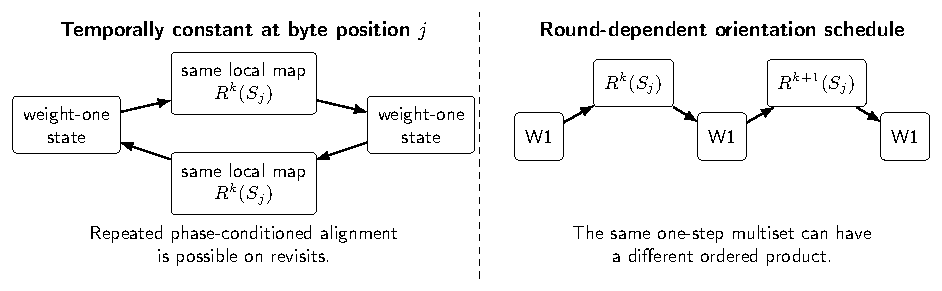
\includegraphics[width=0.96\textwidth]{Fig2_phase_ordering}
\caption{Conceptual illustration of the temporal-alignment interpretation. A temporally constant schedule can present the same oriented byte-local map when a low-support path revisits a position, while a round-dependent schedule changes the map with phase. The schematic is explanatory only: the measured ordering reversal establishes sensitivity to ordered composition, not a unique causal mechanism.}\label{fig:phase-schematic}
\end{figure}

\subsubsection{Linear Squared-Correlation Analogue}\label{sec:3-7-linear}
The mean-field identity has a linear analogue. Let
\[
C(\alpha,\beta)=2^{-8}\sum_x(-1)^{\langle\alpha,x\rangle\oplus\langle\beta,S(x)\rangle}
\]
be the normalized correlation of an 8-bit bijective S-box, in the standard linear-cryptanalysis convention of Matsui and correlation-matrix treatments \cite{ref56,ref5}. For every fixed nonzero output mask $\beta$, Parseval's identity gives
\[
\sum_{\alpha\ne0} C(\alpha,\beta)^2=1,
\]
because $C(0,\beta)=0$ for a bijection and nonzero $\beta$. Summing over the eight weight-one output masks therefore gives
\[
\sum_{\alpha\ne0}\sum_{\mathrm{wt}(\beta)=1} C(\alpha,\beta)^2=8.
\]
Thus a uniform nonzero input mask has mean squared-correlation retention $8/255$, exactly the same null value as the differential mean-probability calculation, and
\[
-\log_2 E[C^2]=\log_2(255/8)=4.994353\ldots\ \text{bits/round}.
\]
The supplementary checker verifies both identities directly for the AES S-box. This is a structural null for linear potential, not a complete linear-hull analysis of the harness; no model-exact multi-round linear transfer claim is made here.

\subsubsection{Class Probability versus Best Single Trail}\label{sec:3-7-3}

The 256-context enumeration also separates the maximum aggregate weight-one class probability from the maximum individual trail probability. At 16 rounds the mean best single-trail log probabilities are $-106.50$ (static), $-106.67$ (position-only), $-106.86$ (rotor), and $-106.70$ (round-only), whereas the corresponding mean class values are $-78.21$, $-78.24$, $-78.51$, and $-78.53$. The corresponding class-minus-single gap is computed separately for each context and then averaged over the panel, giving means of $28.29$, $28.43$, $28.34$, and $28.17$ bits, respectively.

This has a methodological consequence beyond the present harness. Bounding the construction by its best individual differential trail would understate the attainable weight-one recurrence by a factor of approximately $2^{28}$ on average. The schedule can redistribute probability among many individual paths without removing the aggregate class. Analyses of this family should therefore aggregate over trail classes rather than infer recurrence probability from the single best trail alone.

\subsection{Reduced-Round Fixed-Key Calibration}\label{sec:model-calibration}
The Markov transfer model is a surrogate for the fixed-key harness, so the revision includes a direct reduced-round calibration rather than relying on the modelling caveat alone. For four fixed key contexts and eight preselected starting bit differences, $2^{18}$ matched plaintext pairs were evaluated per context/start cell at two rounds under each schedule. The aggregate measured versus model-predicted weight-one probabilities were $1.0785\times10^{-3}$ versus $1.0509\times10^{-3}$ (static), $1.2479\times10^{-3}$ versus $1.0815\times10^{-3}$ (position-only), $1.2220\times10^{-3}$ versus $1.0967\times10^{-3}$ (rotor), and $1.0008\times10^{-3}$ versus $0.9956\times10^{-3}$ (round-only). Aggregation therefore looks broadly comparable at this coarse level.

Cell-level behavior is less benign. After the initial $2^{18}$ calibration had been inspected, four zero-hit cells were selected post hoc for higher-resolution discrepancy checks, with one cell chosen from each schedule arm. They were not a prospectively specified or randomly sampled confirmation set. Their model probabilities range from $7.93\times10^{-4}$ to $1.59\times10^{-3}$. Each selected cell was rerun with $2^{20}$ pairs and again produced zero fixed-key weight-one outcomes. Their one-sided 95\% binomial upper bound is $2.86\times10^{-6}$ per cell, far below the corresponding Markov predictions. These selected reruns therefore demonstrate that large cellwise surrogate-to-harness discrepancies can persist at higher sampling resolution, but they do not estimate how frequently such discrepancies occur across the full context/start grid. The Supplementary Material identifies the context, schedule, starting state, model probability, and observed counts for all four rerun cells. Fixed-key modelling error can thus be much larger than the approximately $0.009$-bit/round schedule separation resolved by the surrogate transfer operator. The model rates are interpreted only as properties of the stated Markov process. The exact support-invariance result does not depend on this calibration.

\section{Experimental SPN Harness and Round Function}\label{sec:4}
The historical HESPN construction is used only as an instrumented 128-bit SPN harness for schedule ablation. Every matched arm uses the same accepted seed matrices, SHA-256-derived round keys, AES S-box, whole-state rotation schedule, routing permutation, and input panels; only the orientation exponent changes. Figure~\ref{fig:design} summarizes the control structure. The complete byte ordering, matrix packing, key setup, encryption and decryption procedures, and reference test vectors are moved to the supplementary material.

\subsection{State Motion and Orientation Schedules}\label{sec:4-1}
The state is 16 bytes in big-endian, MSB-first order. The fixed whole-state rotation schedule is
\[
[7,3,1,5,\;3,1,5,7,\;1,3,5,7,\;7,3,1,5]\ \text{bits}.
\]
Each four-round block sums to 16 bits and the full schedule to 64 bits, so the within-byte offset realigns at four-round boundaries. Routing mode $r\bmod4$ is identity for mode 0 and swaps byte-index bits $0\leftrightarrow1$, $0\leftrightarrow2$, or $0\leftrightarrow3$ in modes 1, 2, and 3. Theorem~\ref{prop:w1closed} concerns only the byte-local matrix step; Proposition~\ref{prop:routing-composition} and the state-motion audit quantify the separate routing geometry.

For byte position $j$, the four schedule arms are static $R^0(S_j)$, position-only $R^{j\bmod4}(S_j)$, round-only $R^{r\bmod4}(S_j)$, and rotor $R^{(r+j)\bmod4}(S_j)$. All accepted seeds satisfy the common invertibility and branch-number conditions of Section~\ref{sec:3-4}. Thus the experiment changes temporal orientation only, not the seed family or any other round component.

\subsection{Round Summary and Deterministic Context Panel}\label{sec:4-2}
A round performs whole-state rotation, round-key XOR, the scheduled byte-local matrix on each byte, AES S-box substitution, and routing, in that order. Round-key XOR is difference-transparent for the transfer analysis. The primary panel uses $K_i=\mathrm{SHA256}(\texttt{HESPN-MATCHED-CONTROL-KEY}\parallel\mathrm{uint32be}(i))$. These master keys are treated as a deterministic pseudorandom panel for reproducibility, not as a distribution-free sample of all admissible matrices. Candidate byte matrices are derived from each key and rejected until the documented invertibility and branch conditions hold; this rejection rule defines the effective matrix ensemble.

Across the 256 primary contexts, 4096 accepted byte seeds required 465,673 candidate draws, for an empirical acceptance fraction of $0.00880$. Contexts required a mean of 1819 candidate draws (median 1798.5; range 667--3225). Per accepted seed the median draw count was 80, the 95th percentile 335.25, and the maximum 843. Panel-prefix and independent-label sensitivity results are reported with the transfer results above and in full in the Supplementary Material. No claim that SHA-256 output constitutes a formal random sample is required for the structural theorem; the panel analysis is conditional on the stated deterministic generation procedure.

\subsection{Evaluation Scope}\label{sec:4-3}
Round counts $4$, $8$, $12$, and $16$ span early structured propagation through later empirical saturation and are observation points, not a proposed security parameter. The harness is not proposed with a deployment mode or authenticated-encryption construction. Its only role is to make the orientation mechanism reproducible and experimentally separable. Full implementation detail is retained in the supplement and repository rather than repeated in the main article.
\section{Matched Evaluation and Boundary Setting}\label{sec:primary}
The exact structural and transfer analyses are primary. The finite empirical instruments are retained only to detect gross behavior that would contradict the structural interpretation; they are not used to estimate the approximately $0.009$-bit/round transfer-model separation.

\subsection{Matched Finite-Resolution Corroboration}\label{sec:5-9}
All four schedules share the same key contexts, accepted matrices, round keys, S-box, state motion, and input panels. The original paired avalanche screen gives a rotor-minus-static mean of $+0.187$ bits at eight rounds with 95\% interval $[-0.131,0.506]$, and the twelve-round counter-distance means differ by only $0.034$ bits across schedules with broadly overlapping intervals. These instruments can exclude only much larger effects than the transfer-model separation. The common counter-stride signature also appears in all schedule arms, supporting the conclusion that this reduced-round geometric feature is not created by the orientation rule. Full avalanche, collision, counter, NIST SP~800-22, and other secondary diagnostic outputs remain in the Supplementary Material; none is used as cryptanalytic security evidence.

\subsection{Exploratory Cross-Byte Boundary Example}\label{sec:5-10}
A separate $4\times4$ Cauchy MDS experiment over $\mathrm{GF}(2^8)$ is retained only to mark where the byte-local support theorem ceases to apply. It changes mixing width, field, and matrix family simultaneously, and its pruned searches remain far from the certified activity floor. It therefore supports no schedule ranking and no causal attribution to width. Detailed candidate tables and audit outputs are confined to the Supplementary Material. A same-field binary layer spanning adjacent bytes would be a cleaner future ablation, but designing and validating that construction is outside the scope of this revision.

\section{Discussion and Conclusions}\label{sec:6}
\subsection{Answer to the Research Question and Design Implication}\label{sec:6-1}
For independently applied byte-local linear maps, changing orientation cannot enlarge active-byte support at the matrix step. That statement is a screening invariant, not a general theorem about cross-byte diffusion layers. The weight-one transfer analysis quantifies what remains after support width is held fixed: coefficient and phase changes can alter the surrogate transition process, but the observed schedule separation is small.

Within the Markov model, the rotor-minus-static periodic-rate difference is about $0.00881$ bits/round on the primary panel and remains of the same order under panel-size and independent-label sensitivity checks. If one nevertheless extrapolates the 16-round class to the fixed-input endpoint reference at the asymptotic rates, rotor shortens the remaining model distance by about $0.076$ of one round. Approximately $0.061$ of that difference is the level gap already present at round 16 and about $0.015$ is attributable to the asymptotic rate difference. This is a model-only extrapolation, not a security gain.

The reduced-round fixed-key calibration sharpens the limitation. Individual context/start cells can depart from the Markov prediction by far more than the transfer-model schedule separation. The numerical result is therefore best read as evidence about the surrogate process and about how coefficient ordering behaves under that model, not as an operational fixed-key differential advantage.

The portable design implication is structural. If a designer wants stronger active-S-box growth, resources should be directed toward a layer or state-motion mechanism that actually couples symbol supports. A public schedule that refreshes coefficients only inside an already active byte may change local transition quality, but it adds no entropy and does not enter a byte-level wide-trail bound. This does not make coefficient variation useless; it places its possible benefit in the narrower category of coefficient-sensitive ordering effects.

The one-step/periodic reversal is consistent with temporal-alignment effects, but the present four-schedule study does not establish phase locking as the unique cause. State-dependent row sums, localization, and other noncommutative effects remain possible explanations. Figure~\ref{fig:phase-schematic} is therefore conceptual rather than causal evidence.

\subsection{Generality Beyond the AES S-box}\label{sec:6-generality}
The byte-local support invariant is independent of the S-box: it is a support statement about any independently applied byte-local linear map. The minimum-support interpretation likewise extends to SPNs with one bytewise S-box per active byte. The differential mean-field identity is also broader than AES. For every bijective 8-bit S-box, each nonzero DDT output column has total mass 256 across nonzero input differences, so the average probability of landing in one of eight weight-one outputs is exactly $8/255$. The Parseval argument gives the same $8/255$ mean squared-correlation null for any bijective 8-bit S-box.

What is S-box-specific is the distribution around those means and therefore the actual finite and periodic rates induced by the scheduled matrix images. The magnitude of the phase-ordering effect reported here should not be transferred numerically to another S-box, matrix family, routing rule, or state-motion schedule without recomputation. The general claim is narrower and stronger: coefficient variation within fixed byte-local support cannot directly create diffusion width, while the average differential and linear nulls arise from bijectivity rather than from an AES-specific coincidence.

\subsection{Why Trail-Class Aggregation Matters}\label{sec:6-trailclass}
The mean per-context log-domain gap between the aggregate weight-one class and the best single trail is about $28$ bits across the deterministic panel. This is a methodological observation rather than a probability ratio formed from arithmetic means. In designs that admit recurrent low-support behavior, bounding only the most probable trail can substantially understate the probability mass accumulated across many related trails. The present finite-state class is narrow and does not replace a full hull computation, but it demonstrates why class aggregation should accompany single-trail bounds when the geometry permits repeated return to a low-support state set.

\subsection{Routing Localization}\label{sec:6-routing}
The twelve-round counter-distance deficit provides an independent localization result. Proposition~\ref{prop:routing-composition} proves that the isolated routing sequence has an order-four four-round composition, while the rotation schedule realigns within-byte bit offsets after each four-round block. The counter experiment confirms the same stride signature in all four matrix-schedule arms. A separate state-motion-only checker shows that composing the actual whole-state rotations with routing has order $504$ over four rounds and $60{,}060$ over sixteen, under either rotation-direction convention. Thus the small order is a routing-layer property that rotation destroys; it should not be interpreted as a short period of the complete state motion. The common stride signature remains independent of matrix orientation.

\subsection{Cross-Byte Boundary and Open Questions}\label{sec:6-2}
The cross-byte MDS experiment marks the boundary of Theorem~\ref{prop:w1closed}: once the linear map connects several byte positions, the byte-local support proof no longer applies. The current beam searches are too far from the certified activity floor to establish a schedule ranking, and the intervention also confounds width, field, and matrix family. The useful conclusion is therefore prospective. A same-field binary map spanning two adjacent bytes is the natural next control because it changes support geometry while preserving more of the original algebraic setting.

Other structural questions follow directly: examine routing families whose four-round composition does not have small order; extend the transfer analysis beyond the weight-one differential class and toward linear hulls; characterize how periodic schedule phases couple to S-box transition structure; and design schedule objectives aligned with cryptanalytic quantities rather than generic diffusion surrogates. These questions test mechanisms that can alter support growth rather than merely adding coefficient diversity.

\subsection{Limitations}\label{sec:6-4}
The transition enumeration is exact only within Remark~\ref{rem:markov}; it covers the weight-one iterative class, not the complete differential or linear hull of a fixed keyed permutation. The 256-context panel is deterministic and its population interpretation depends on treating the SHA-256-derived keys as a pseudorandom panel under the documented rejection rule. The independent-label replication tests sensitivity to that label but does not convert the study into a distribution-free proof. Fixed-key calibration shows that modelling error can exceed the schedule separation. The empirical diagnostics are intentionally secondary, and the cross-byte search is exploratory and pruned. None of these results constitutes a security proof for the complete experimental permutation.

\subsection{Reproducibility}\label{sec:6-3}
The primary byte-local matched-control results are reproduced by
{\footnotesize\path{matched_orientation_schedule_experiment.py}}. The runner verifies the rotor arm
against the supplementary reference vector before running. The cross-byte boundary study is
provided under \path{src/cross_byte/} in the public repository snapshot. Its unit
tests verify all four MDS orientations, encryption/decryption round trips, schedule
periods and structural audits. The validated standard-profile outputs include the
MILP activity bounds, capped minimum-support counts, differential and linear
candidate tables, captured low-active mass, schedule-optimizer record, and compact
slide/reflection summary. Full pair lists remain available in the archival audit
JSON.
\supplementary{The following supporting information accompanies this article: Supplementary Technical Material; Supplementary Code and Results. The files contain the validated byte-local matched-control implementation, the 256-context transition and periodic-transfer analysis with machine-readable outputs, matched statistical diagnostics, cross-byte MDS candidate and audit tables, trail-search code, sensitivity analysis, reference implementation, test vectors, and a reproducibility manifest.}

\authorcontributions{Conceptualization, P.E.C.; methodology, P.E.C.; software, P.E.C.; validation, P.E.C.; formal analysis, P.E.C.; investigation, P.E.C.; resources, P.E.C.; data curation, P.E.C.; writing---original draft preparation, P.E.C.; writing---review and editing, P.E.C.; visualization, P.E.C. The author has read and agreed to the published version of the manuscript.}

\funding{This research received no external funding.}

\institutionalreview{Not applicable.}

\informedconsent{Not applicable.}

\dataavailability{The source code and machine-readable outputs supporting the transfer analysis, panel-sensitivity and starting-state checks, numerical validation, reduced-round fixed-key calibration, matched empirical controls, and exploratory cross-byte boundary experiment are included in the supplementary submission package and maintained in the public GitHub repository at \url{https://github.com/ja9925ydbsu/structural-limits-orientation-scheduling}. The supplementary manifest maps manuscript tables to scripts and output files. No third-party datasets were used.}

\acknowledgments{During the preparation of this manuscript, the author used Anthropic Claude and OpenAI ChatGPT to assist with Python refinement, copy editing, manuscript review, table and figure assembly, and reference formatting. The author independently verified the code and all reported measurements, reviewed and edited the outputs, and takes full responsibility for the content of this publication.}

\conflictsofinterest{The author declares no conflicts of interest.}

\abbreviations{Abbreviations}{%
The following abbreviations are used in this manuscript:\\

\noindent
\begin{tabular}{@{}ll}
AES & Advanced Encryption Standard\\
DDT & Difference Distribution Table\\
GF & Galois field\\
MDS & Maximum distance separable\\
SPN & Substitution-permutation network
\end{tabular}}

\begin{adjustwidth}{-\extralength}{0cm}
\reftitle{References}
\bibliography{references}
\PublishersNote{}
\end{adjustwidth}
\end{document}
